
\section{Taylor-Polynome} \label{MA2-taylorpolynome}

\begin{table}[H]
  \centering
  \begin{tabularx}{\textwidth}{@{}>{\raggedright\arraybackslash}X r@{}}
    \toprule
    \multicolumn{2}{c}{\textbf{�bersicht �ber Lernziele und Voraussetzungen}}\\
    \midrule
    \textbf{Lernziele} & \\[.5\normalbaselineskip]
    \tabitem Taylor-Polynome $p_n$ einer Funktion am Entwicklungspunkt $x_0$ berechnen & \\
    \midrule
    \textbf{Voraussetzungen} & \\[.5\normalbaselineskip]
    \tabitem das Konzept der linearen N�herung (Tangentengerade) &  \abschnittsverweis{MA1-stetigkeit-und-differenzierbarkeit}\\
    \tabitem Ableitungen (inkl.\ h�herer Ableitungen) bilden &  \abschnittsverweis{MA1-ableitungsregeln}  \\
    \bottomrule
  \end{tabularx}
\end{table}

\noindent \ifintegriereaufgaben Die �bungsaufgaben zum Thema finden Sie \hyperref[MA2-taylorpolynome-aufgaben]{hier}.
\vspace{0.3cm}
\hrule
\fi


Gegeben sei eine \underline{differenzierbare}\randverweis{MA1-ableitungsregeln} Funktion $f: D_f \to \mathbb R$. Dann kann man die Gerade suchen, welche $f$ an einer Stelle $x_0\in D_f$ am besten ann�hert\footnote{im Sinne einer Interpolation bz�glich Funktion und Ableitung!}: das ist die \underline{lineare N�herung}\randverweis{MA1-stetigkeit-und-differenzierbarkeit} oder auch Tangentengerade.
\begin{exabox}{Tangentengerade}{ }
	\hspace{-0.3cm}\begin{minipage}{0.4\textwidth}
		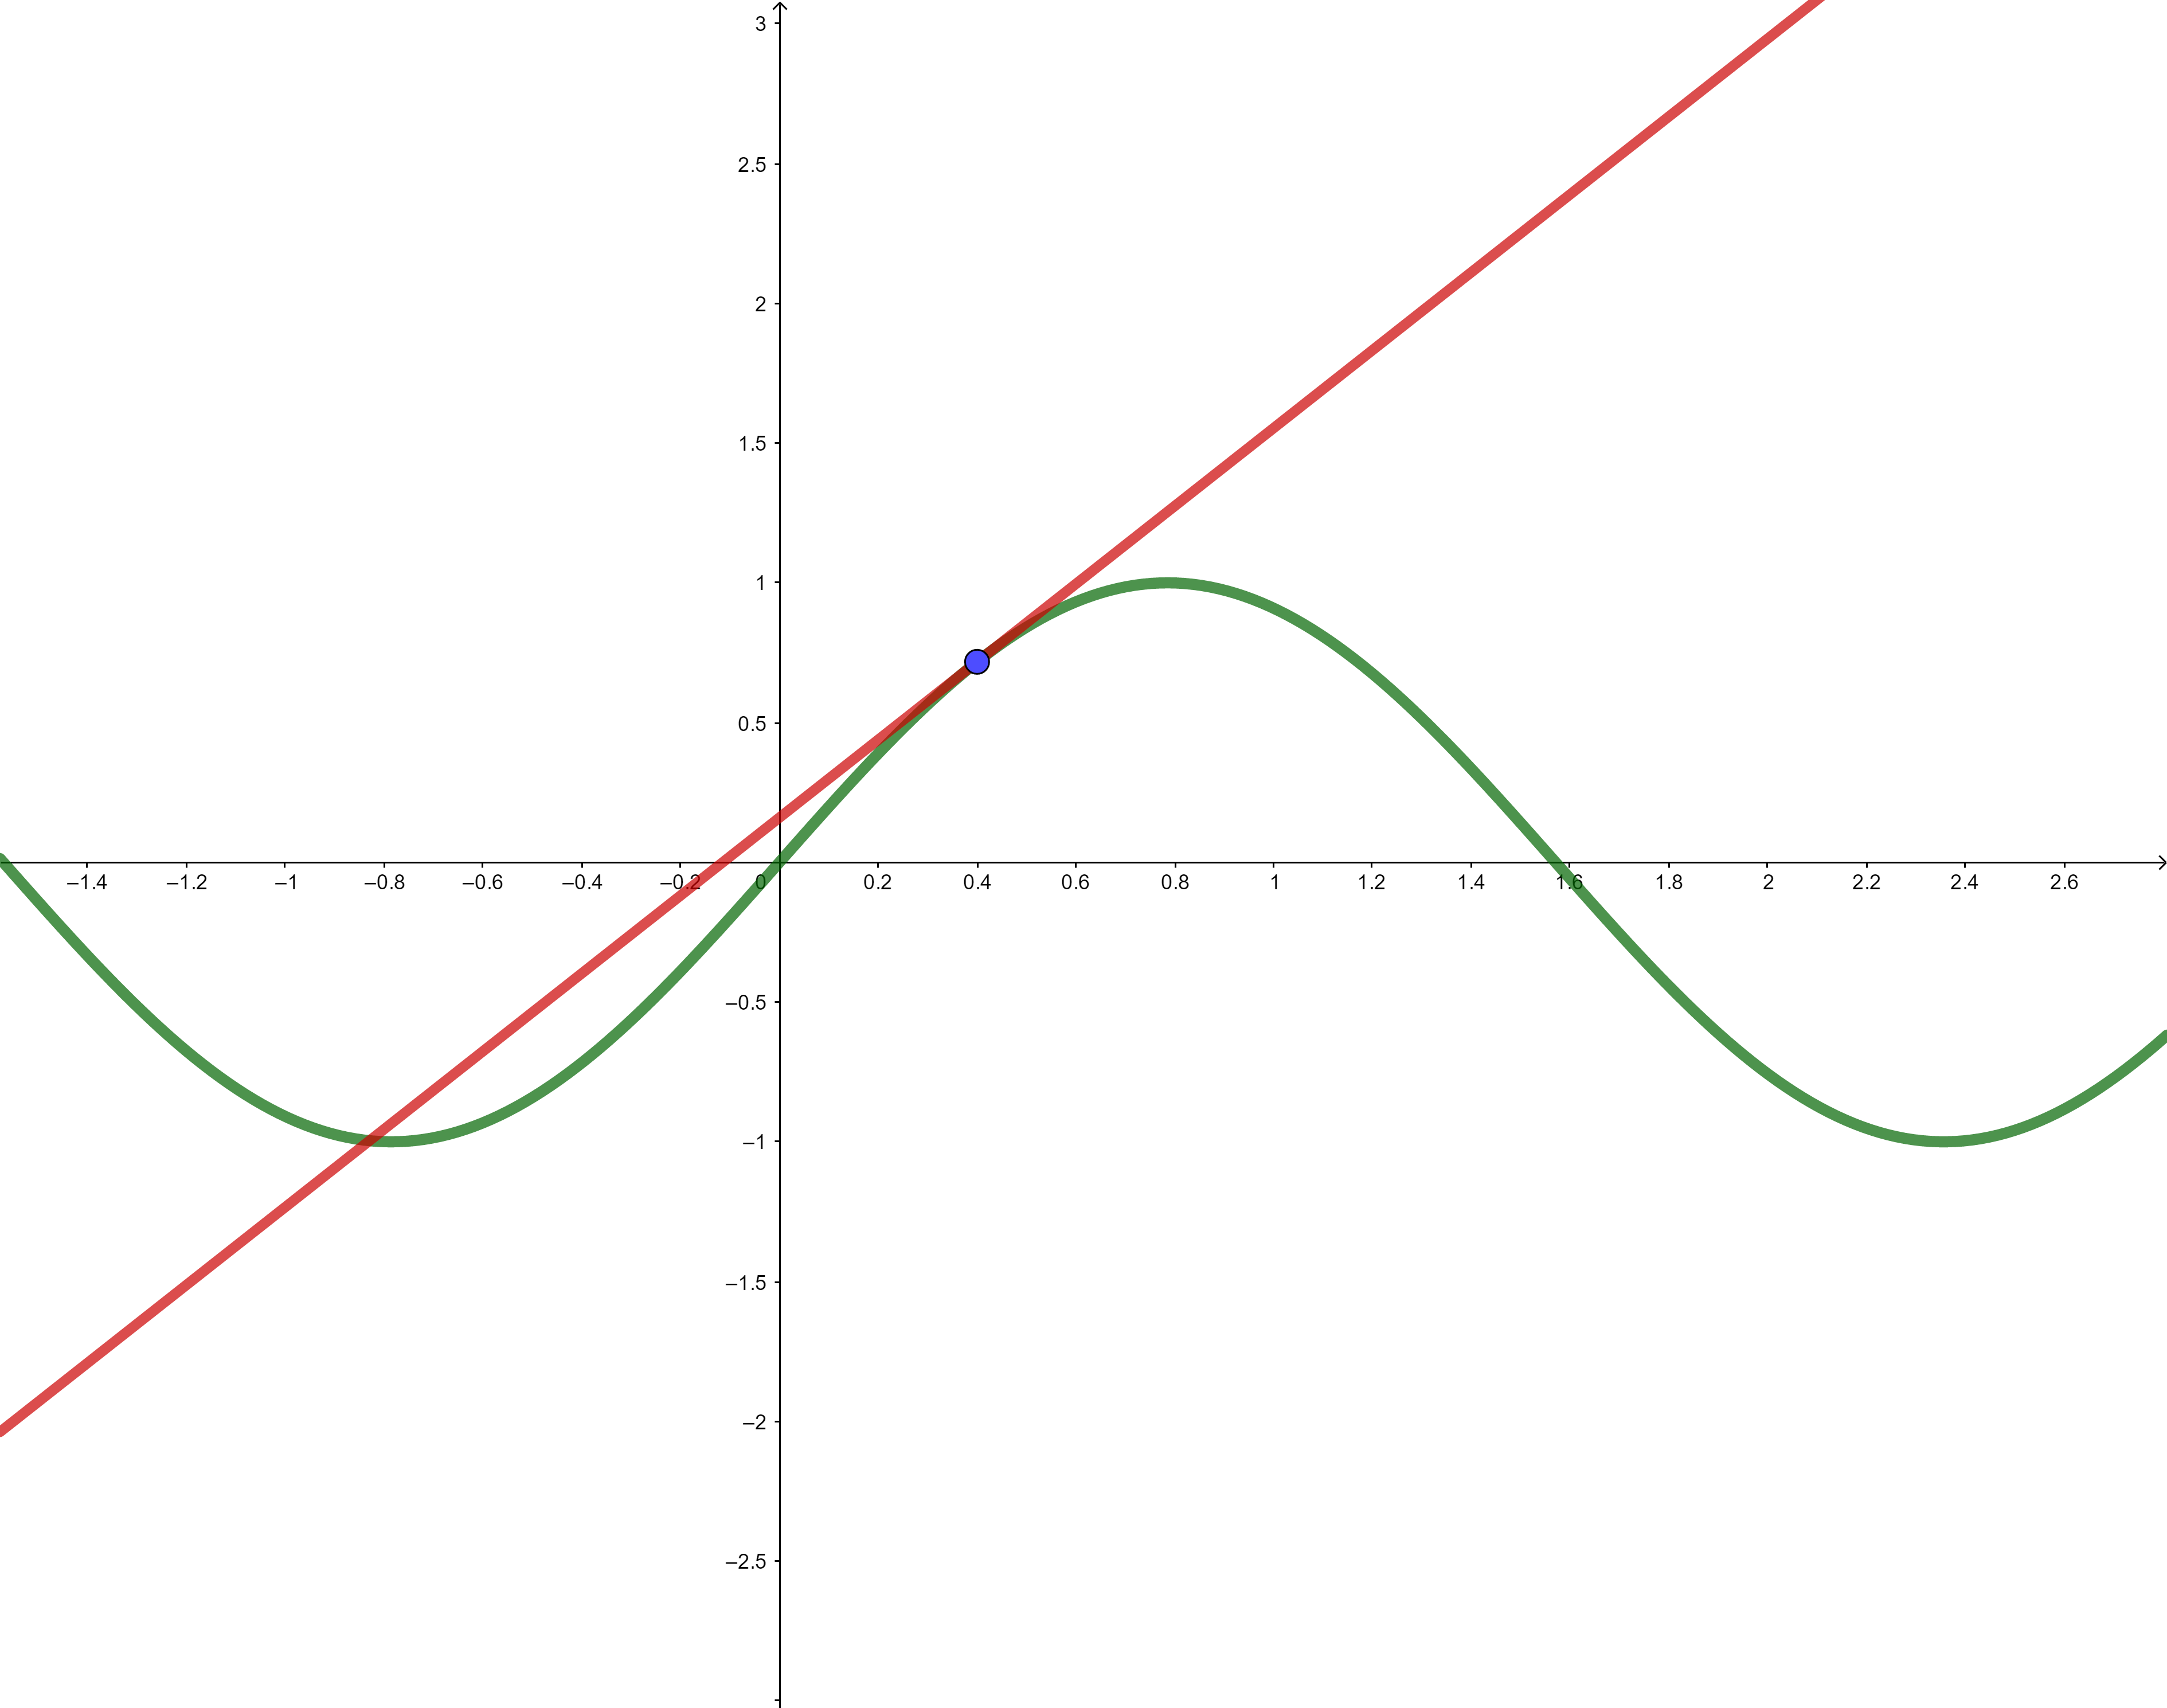
\includegraphics[width=\textwidth]{../Mathematik_2/Bilder/taylor_sinus_tangente.png}
\end{minipage}
	\begin{minipage}{0.6\textwidth}
		F�r $\sin:x\mapsto \sin(x)$ lautet die Tangente in $x_0=2/5$: \[p_1:x\mapsto \sin(2/5) + \cos(2/5)(x-2/5)\]
		Die Tangente erf�llt:
	\begin{itemize}
		\item $p_1(2/5) = \sin(2/5)$ ,
		\item $p_1'(2/5) = \cos(2/5)$.
	\end{itemize}
\end{minipage}
\end{exabox}

F�r eine beliebige differenzierbare Funktion lautet die Tangentengerade an der Stelle $x_0$ also
\[
	p_1(x) =  f(x_0) + f'(x_0)(x-x_0)\,,
\]
und es gilt
\begin{itemize}
	\item $p_1$ l�uft durch den Punkt $(x_0|f(x_0))$, also $p_1(x_0) = f(x_0)$,
	\item $p_1$ hat in $x_0$ dieselbe Steigung wie $f$, also $p_1'(x_0) = f'(x_0)$.
\end{itemize}

Als n�chstes kann man die quadratische Parabel suchen, die sich einer zweimal differenzierbaren Funktion $f$ an einer Stelle $x_0$ am besten ann�hert\footnote{im Sinne einer Interpolation.}: das ist die quadratische N�herung oder auch Schmiegeparabel.
\begin{exabox}{Schmiegeparabel}{ }
	\hspace{-0.3cm}\begin{minipage}{0.4\textwidth}
		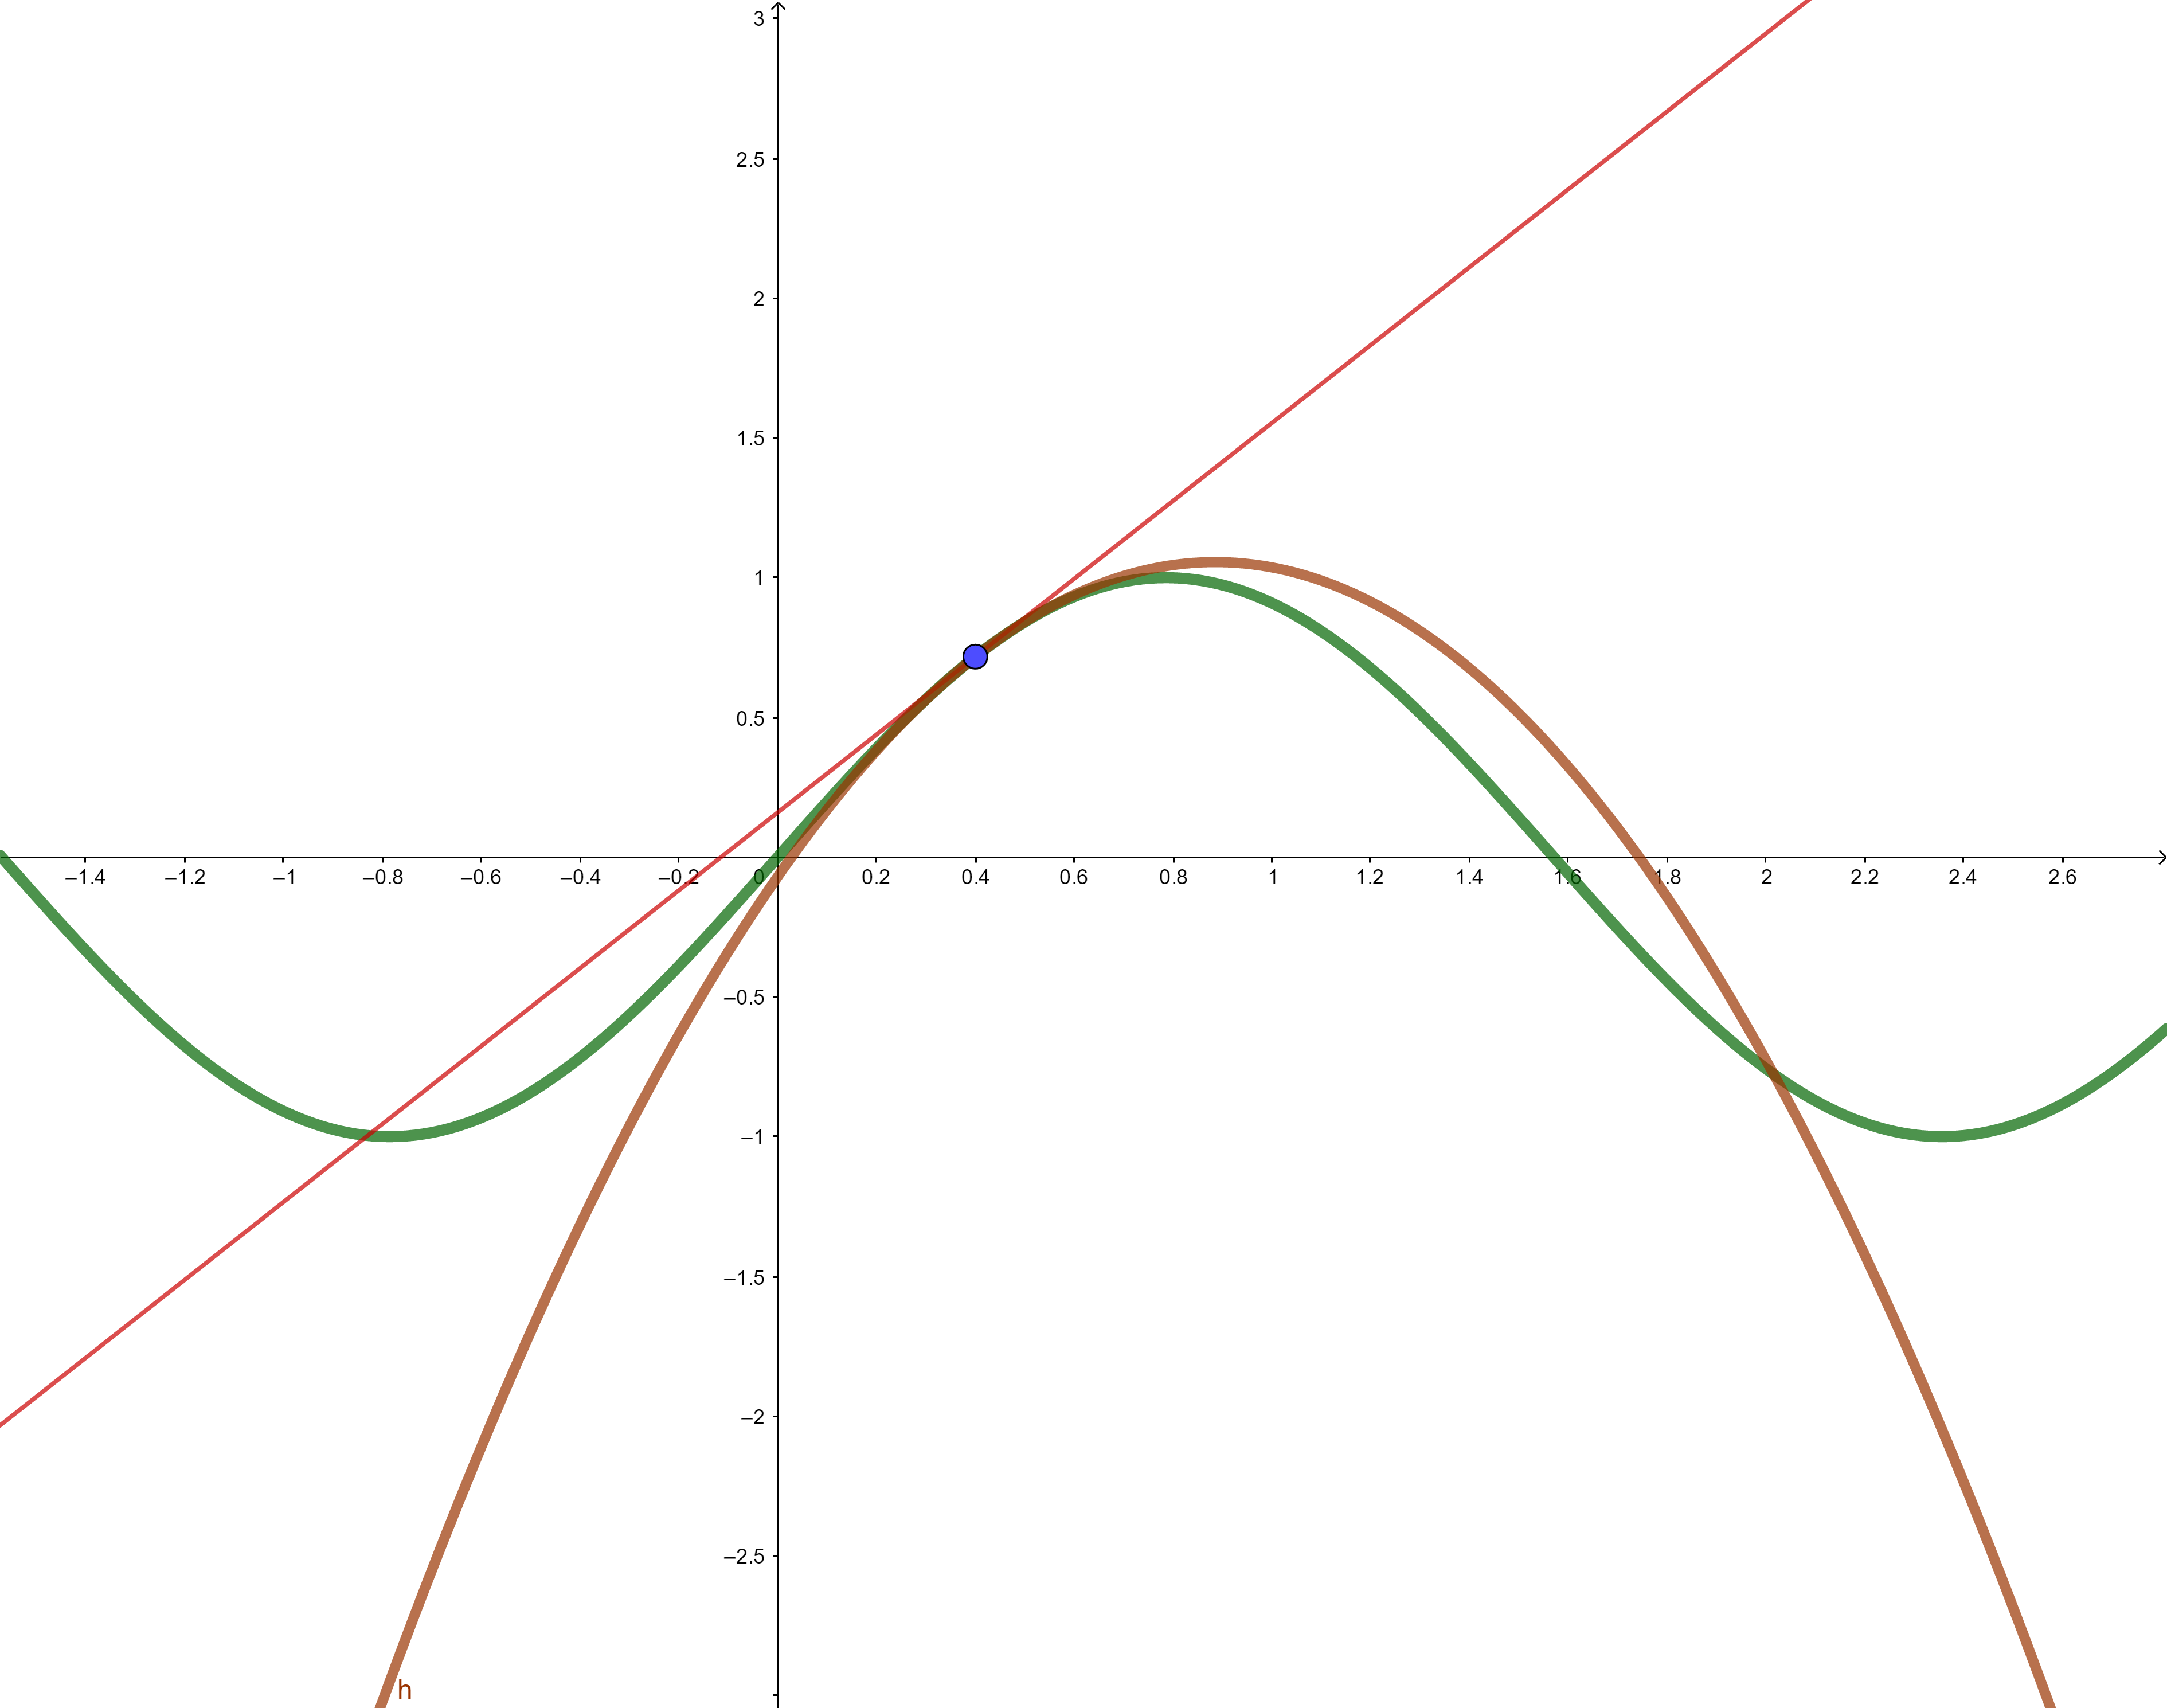
\includegraphics[width=\textwidth]{../Mathematik_2/Bilder/taylor_sinus_schmiegeparabel.png}
\end{minipage}
	\begin{minipage}{0.6\textwidth}
		F�r $\sin:x\mapsto \sin(x)$ lautet die Schmiegeparabel in $x_0=2/5$: \[p_2:x\mapsto \sin(2/5) + \cos(2/5)(x-2/5) - 1/2\sin(2/5)(x-2/5)^2\]
		Die Schmiegeparabel erf�llt:
	\begin{itemize}
		\item $p_2(2/5) = \sin(2/5)$ ,
		\item $p_2'(2/5) = \cos(2/5)$.
		\item $p_2''(2/5) = -\sin(2/5)$.
	\end{itemize}
\end{minipage}
\end{exabox}

F�r eine beliebige zweimal differenzierbare Funktion lautet die Schmiegeparabel an der Stelle $x_0$:
\begin{eqnarray*}
	p_2(x) &=&  f(x_0)+ f'(x_0)(x-x_0) +\frac12 f''(x_0)(x-x_0)^2,
\end{eqnarray*}
und es gilt
\begin{itemize}
	\item $p_2$ l�uft durch den Punkt $(x_0|f(x_0))$, also $p_2(x_0) = f(x_0)$,
	\item $p_2$ hat in $x_0$ dieselbe Steigung wie $f$, also $p_2'(x_0) = f'(x_0)$.
	\item $p_2$ hat $x_0$ dieselbe Kr�mmung wie $f$, also $p_2''(x_0) = f''(x_0)$.
\end{itemize}

Entsprechend  findet  man  die  Formeln  f�r  die beste lokale N�herung durch \underline{Polynome}\randverweis{MA1-polynome} dritten \ldots oder zehnten Grades:
\begin{eqnarray*}
	p_3(x) &=& f(x_0) + f'(x_0)(x-x_0)+ \frac12 f''(x_0)(x-x_0)^2+\frac16 f'''(x_0)(x-x_0)^3\,,\\
	\cdots&&\\
	p_{10}(x) &=& f(x_0) + f'(x_0)(x-x_0)+ \frac12 f''(x_0)(x-x_0)^2+ \cdots + \frac{1}{10!} f^{(10)}(x_0)(x-x_0)^{10}\,.
\end{eqnarray*}

\begin{exabox}{Taylor-Polynom vom Grad $10$}{ }
	\begin{center}
	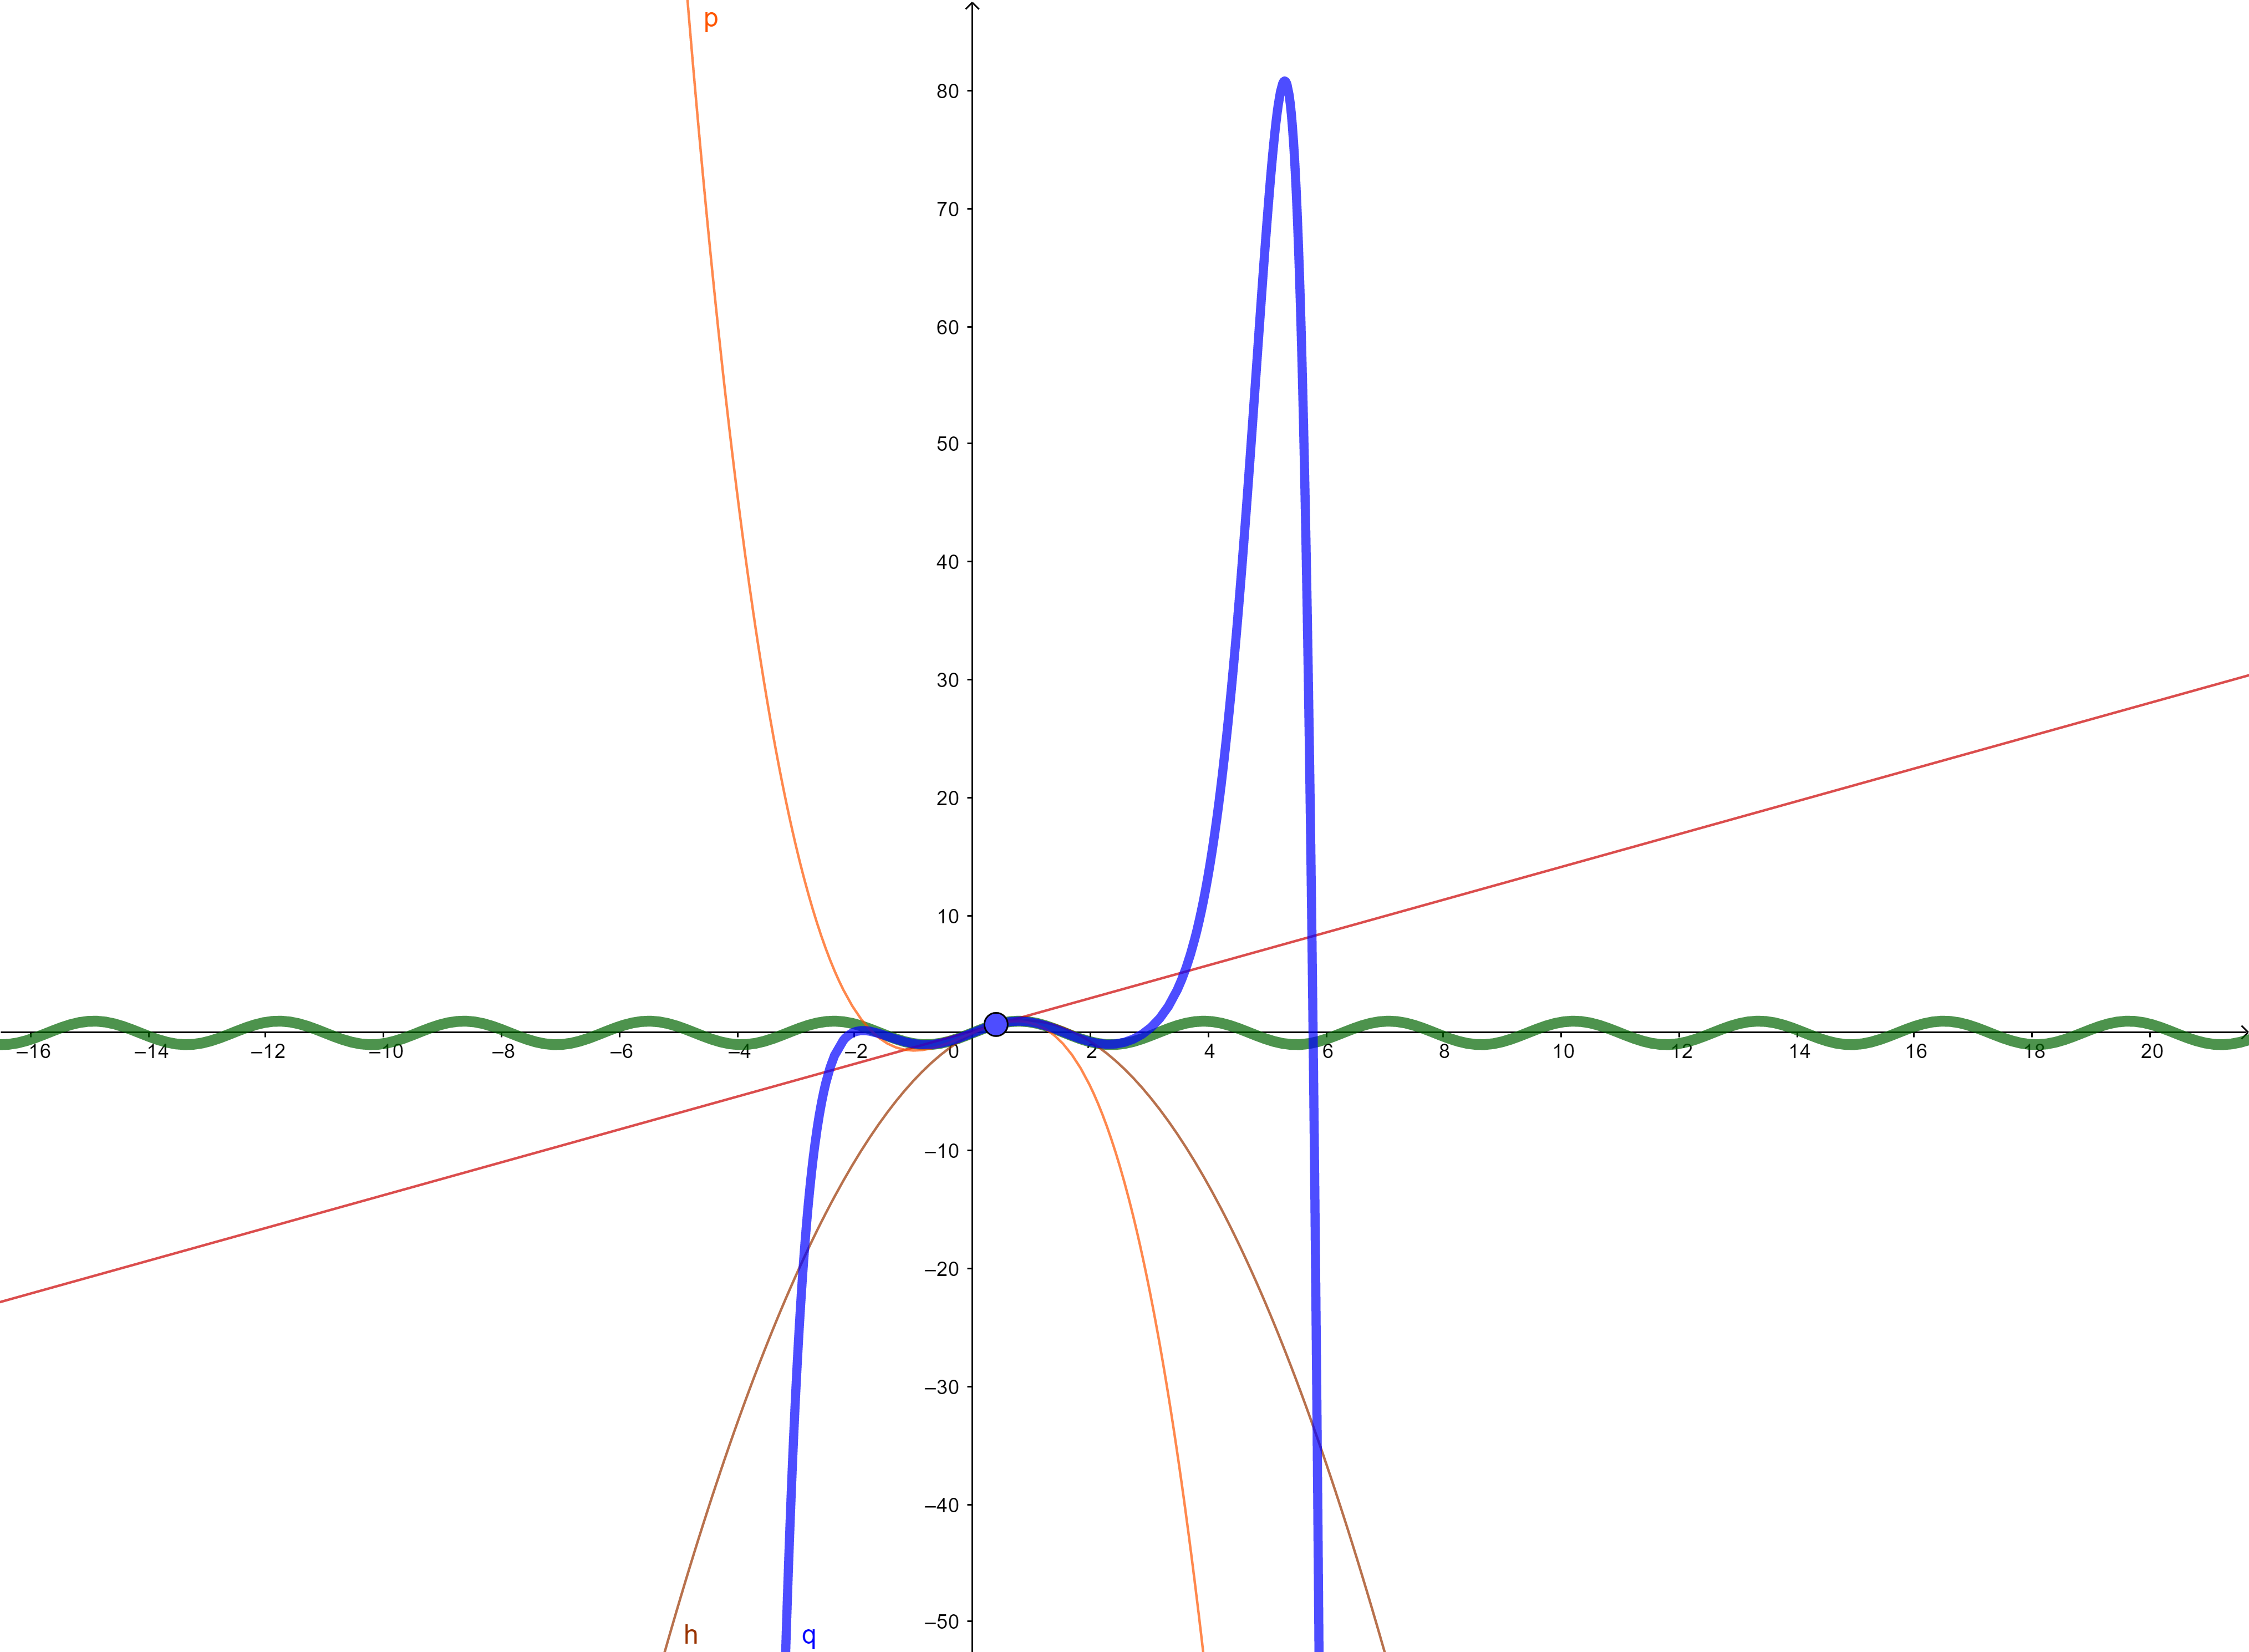
\includegraphics[width=0.7\textwidth]{../Mathematik_2/Bilder/taylor_sinus_polynom_grad_10.png}
\end{center}
\end{exabox}
Vorausgesetzt die Funktion $f$ besitzt mindestens Ableitungen bis zur Ordnung $n$, dann kann man auf diese Weise ein Polynom $p_n$ vom Grad $n$ entwickeln, das sogenannte Taylor-Polynom vom Grad $n$:
\begin{defbox}{Taylor-Polynom vom Grad $n$}{ }
	F�r eine $n$-mal differenzierbare Funktion lautet das Taylor-Polynom vom Grad $n$:

	\begin{eqnarray*}
		p_n(x) &=& f(x_0) + f'(x_0)(x-x_0) + \frac12 f''(x_0)(x-x_0)^2 + \cdots + \frac{1}{n!} f^{(n)}(x_0)(x-x_0)^n \\
		&=& \sum\limits_{k=0}^{n}\frac{1}{k!}f^{(k)}(x_0)(x-x_0)^k\,.
\end{eqnarray*}
Das Taylorpolynom $p_n$ stimmt an der Stelle $x=x_0$ mit der Funktion $f$ und mit deren Ableitung bis zum Grad $n$ �berein:
\[ \forall\, k=0,\cdots,n: \quad p_n^{(k)}(x_0)= f^{(k)}(x_0)\,.  \]
\end{defbox}

\noindent Bemerkungen:\marginpar{\small Aufgaben}
\begin{itemize}
	\item In der Praxis ist nur das lokale Verhalten einer Funktion oder Kennlinie interessant. Um die Analyse zu erleichtern kann man anstatt der Orginalfunktion ein Taylorpolynom betrachten!
	\item Das \underline{asymptotische Verhalten}\randverweis{MA1-ableitungen-und-funktionsverlauf} des Taylorpoynoms entspricht dem des Polynoms und kann unter Umst�nden ganz anders sein als das der betrachteten Funktion!
	\item Wechselt man den Entwicklungspunkt $x_0$, muss man das Taylorpolynom neu bestimmen.
\end{itemize}

Im folgenden Beispiel wird die Wurzelfunktion an der Stelle $x_0 = 4$ mit einem Taylorpolynom vom Grad $3$ angen�hrt:
\begin{exabox}{Taylor-Polynom an $f:x\to\sqrt{x}$ vom Grad $n=3$ an $x_0=4$}{ }
Bestimmung der Ableitungen bis zum Grad $3$:
\begin{eqnarray*}
		f(x) &=& \sqrt{x} = x^{1/2}\,,\\[1ex]
		f'(x) &=& \frac12 x^{-1/2} = \frac12 \frac{1}{\sqrt{x}}\,,\\[1ex]
		f''(x) &=& -\frac14 x^{-3/2} =- \frac14 \frac{1}{\sqrt{x}^3}\,,\\[1ex]
		f'''(x) &=& \frac38 x^{-5/2} =- \frac38 \frac{1}{\sqrt{x}^5}\,.
	\end{eqnarray*}

L�sung $p_3$ mit $x_0=4$:
	\[
	p_3:\mathbb R \to \mathbb R, x\mapsto 2 + \frac14(x-4)- \frac{1}{32} \frac{1}{2} (x-4)^2 + \frac{3}{256} \frac{1}{6} (x-4)^3\,.
\]
\begin{center}
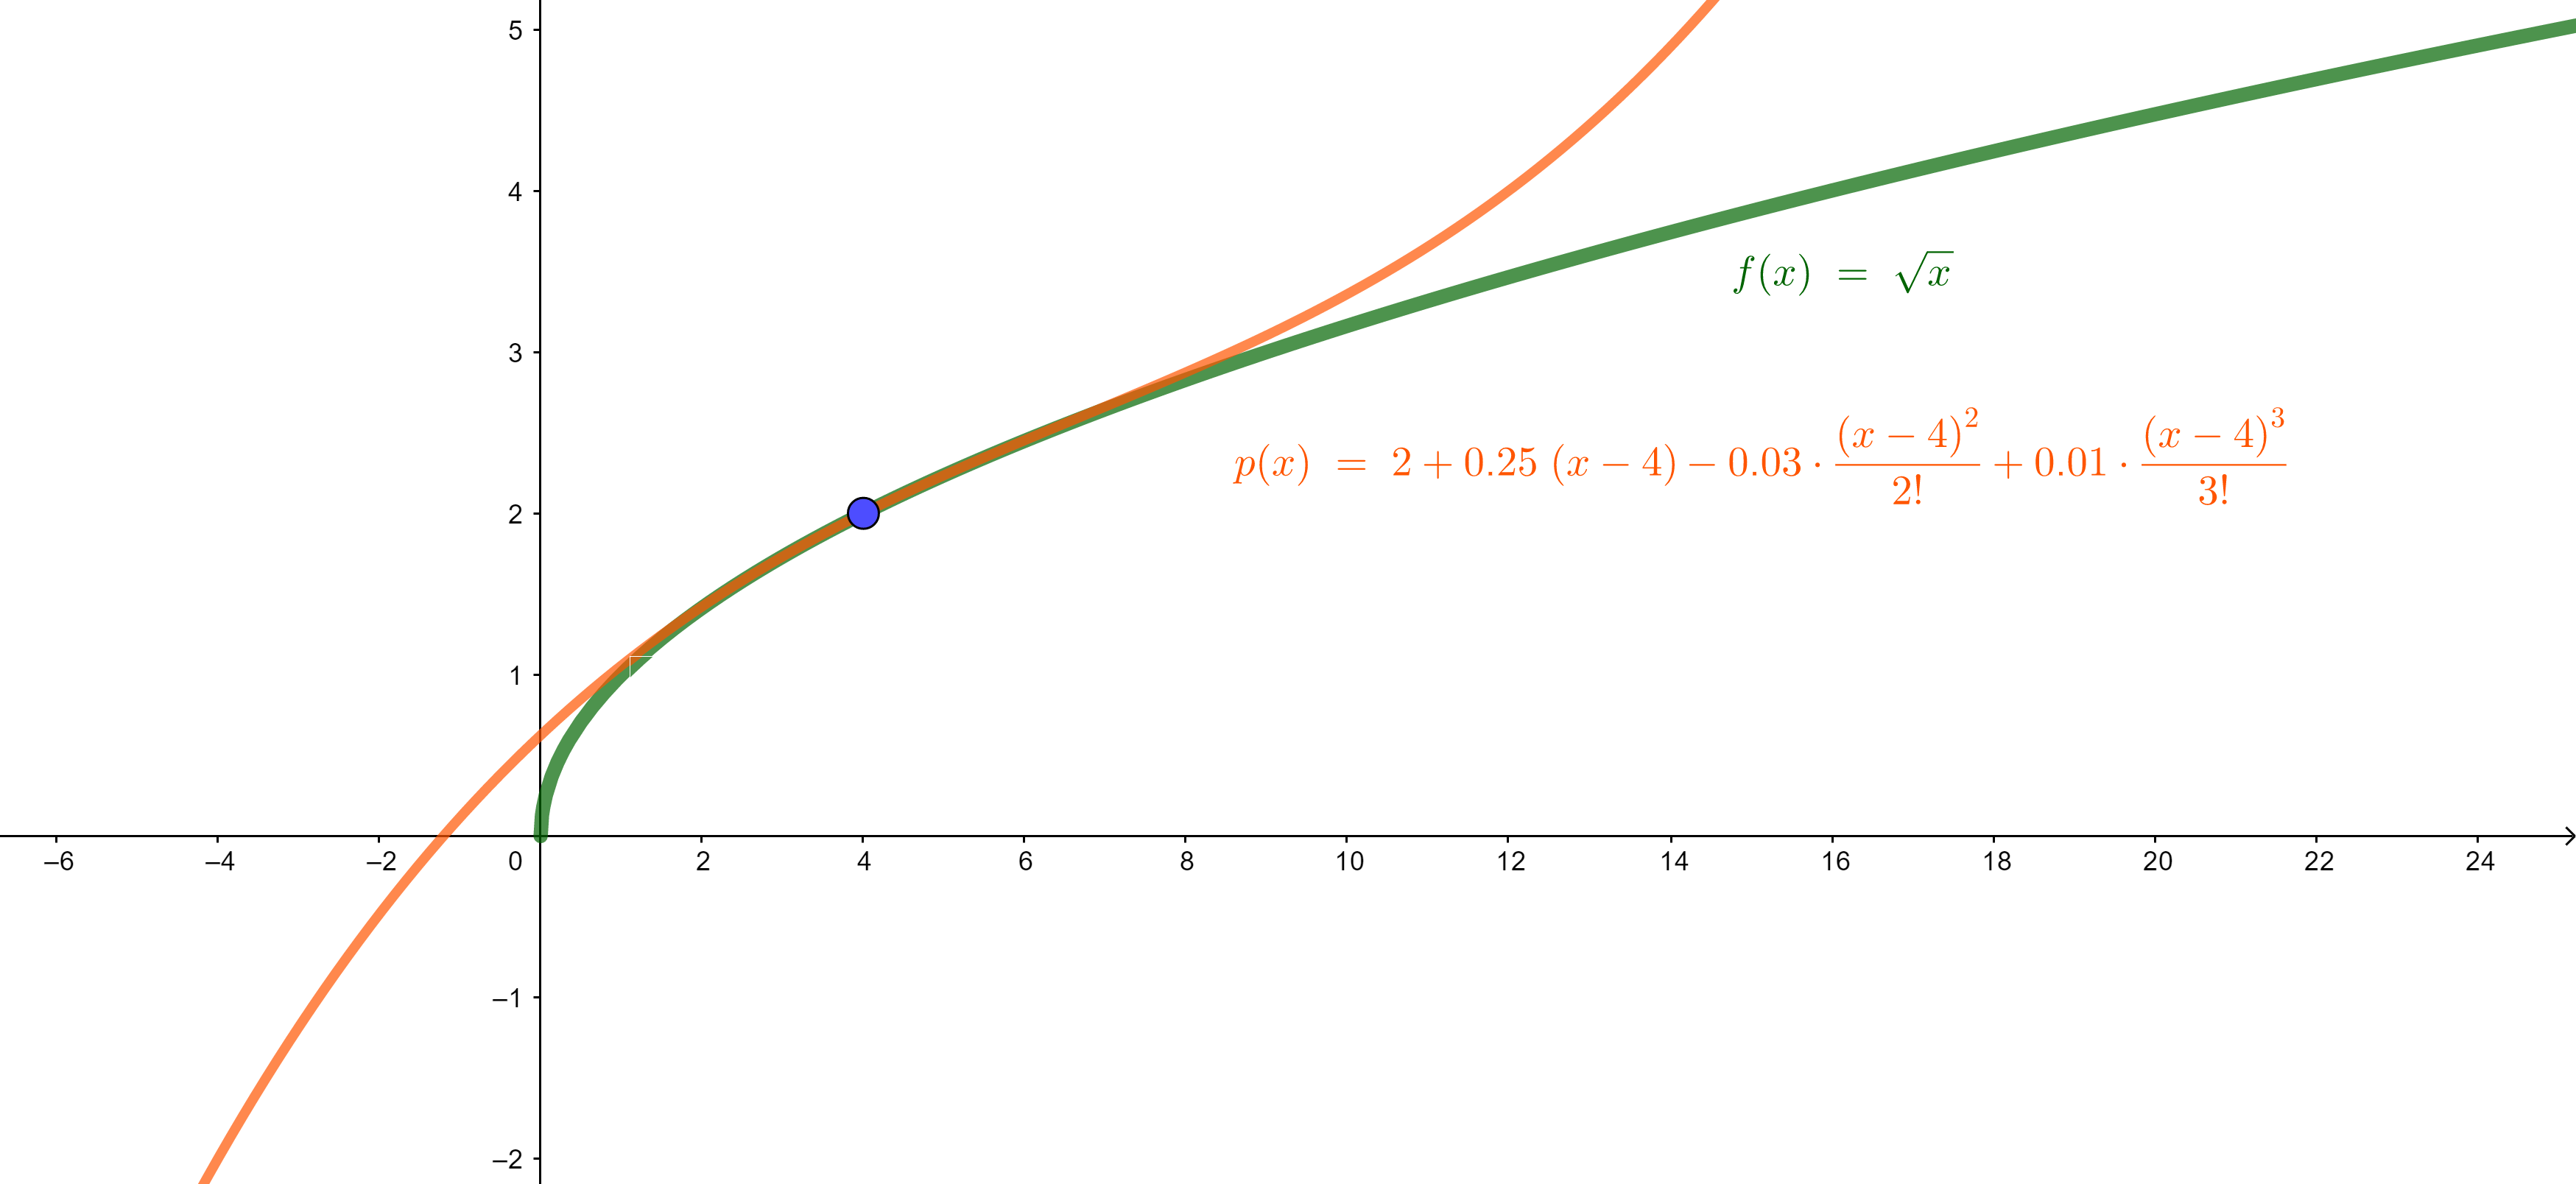
\includegraphics[width=0.7\textwidth]{../Mathematik_2/Bilder/taylor_wurzelfunktion_polynom_grad_3.png}
\end{center}
\end{exabox}

